%-----------------------------------------------------------------
%	SST ANALYSIS
%	!TEX root = ./../main.tex
%-----------------------------------------------------------------
\subsection{SST analysis}\label{sec:sst-analysis}
In figures~\ref{fig:sst-analysis-natl} and~\ref{fig:sst-analysis-epac} we can see the result of doing the analysis described in~\cref{ssec:hadisst-import} using the function \inline{plot_annual_sst()} defined in the script~\ref{scr:hadisst_base} in~\cref{app:code}. The spatial and temporal activity windows used are the ones described in table~\ref{tab:act-windows}.
\begin{figure}[H]
	\centering
	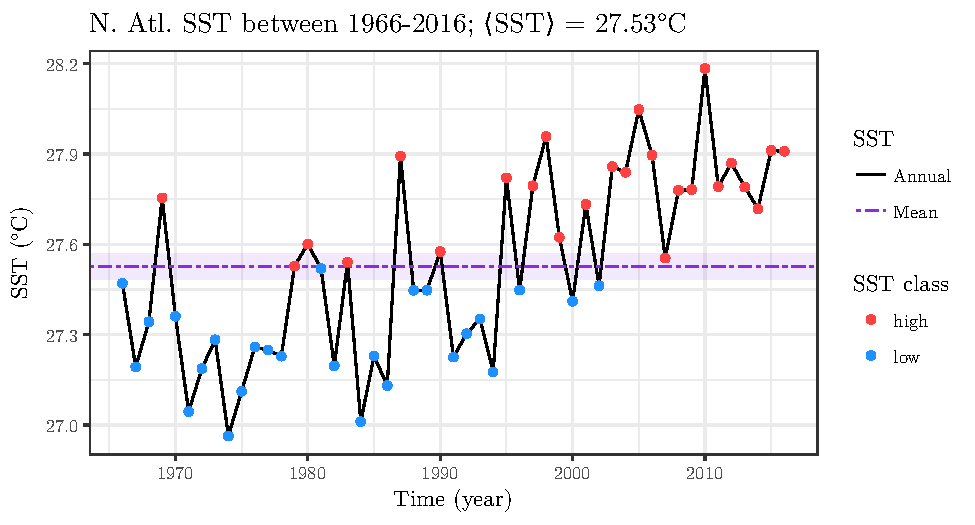
\includegraphics[width=0.99\textwidth]{images/sst-analysis-natl}
	\caption{SST analysis for the North Atlantic Ocean}
	\label{fig:sst-analysis-natl}
\end{figure}

\begin{figure}[H]
	\centering
	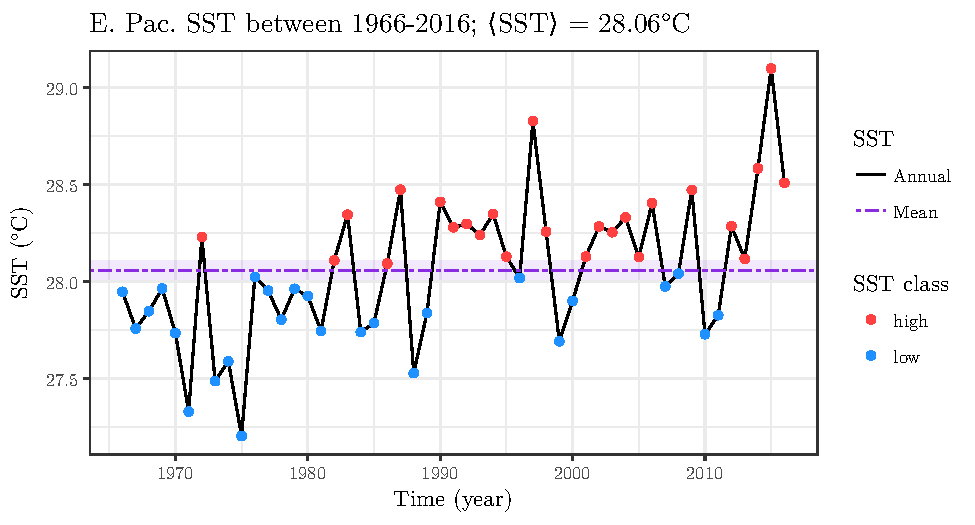
\includegraphics[width=0.99\textwidth]{images/sst-analysis-epac}
	\caption{SST analysis for the Northeast Pacific Ocean}
	\label{fig:sst-analysis-epac}
\end{figure}

The first thing we notice is the general tendency of increasing sea surface temperatures after the 1970s (being the year 1975 a reasonable estimation of the \emph{start} of global warming; see figure~\ref{fig:global-temps}), and an alarming increase in the rate of warming after the 2000s.

In table~\ref{tab:sst-evolution} we can see the evolution of $\ev{\text{SST}}$ comparing three time periods starting from the year 1966: (i) years before the global warming, (ii) years studied in \citeauthor{Corral2010}'s original text, and (iii) years studied in this text. As shown, the increase in the sea surface temperatures is quite noticeable.
\begin{table}[H]
	\centering
	\begin{tabular}{l c c c}
		\toprule
		\toprule
		Basin   & 1966--1975 $\ev{\text{SST}}$ & 1966--2007 $\ev{\text{SST}}$ & 1966--2016 $\ev{\text{SST}}$ \\
		\midrule
		N.~Atl. & \SI{27.27}{\celsius} & \SI{27.45}{\celsius} & \SI{27.52}{\celsius} \\
		E.~Pac. & \SI{27.71}{\celsius} & \SI{28.01}{\celsius} & \SI{28.06}{\celsius} \\
		\bottomrule
	\end{tabular}
	\caption{Change of the seasonal mean sea surface temperature}
	\label{tab:sst-evolution}
\end{table}

\begin{figure}[H]
	\centering
	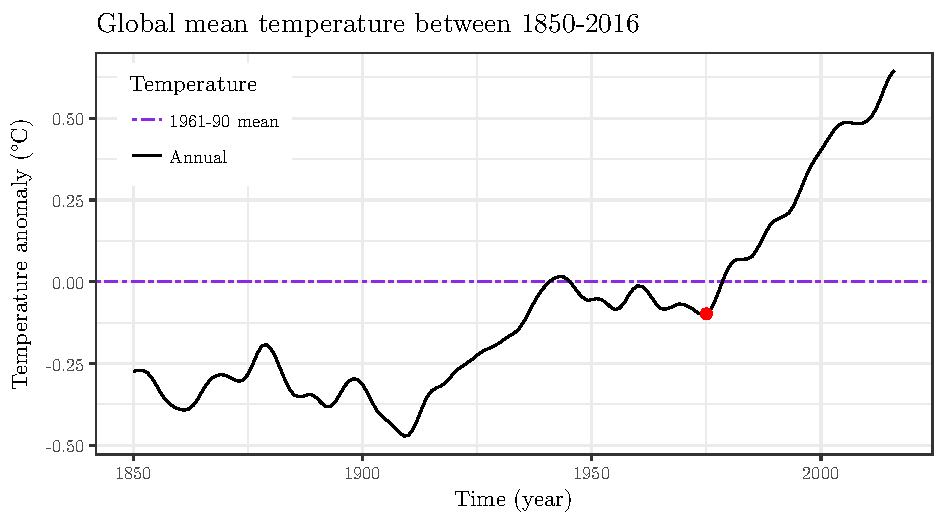
\includegraphics[width=\textwidth]{images/global-temps}
	\caption{Global surface temperature record for the last 166 years}
	\label{fig:global-temps}
\end{figure}

The time series seen in figure~\ref{fig:global-temps}, a reproduction of the global time series from~\cite{o:hadcrut4-diagnostics}, has been created using the data provided by the Met Office's HadCRUT4 database. The data set can be downloaded from \url{http://www.metoffice.gov.uk/hadobs/hadcrut4/data/current/time_series/HadCRUT.4.5.0.0.monthly_ns_avg.txt}.

\sk
In table~\ref{tab:sst-years} we can see the list of years obtained in each one of the basins studied separated by SST class. With this, we have every piece needed to answer the hypothesis raised in~\cref{ssec:dpdi}.
\begin{table}[H]
	\centering
	\resizebox{\textwidth}{!}{%
	\begin{tabularx}{1.05\textwidth}{l c X}
		\toprule
		\toprule
		Basin   & SST class & List of years \\
		\midrule
		\multirow{4}{*}{N.~Atl.} & \multirow{2}{*}{Low}  & 1966 1967 1968 1970 1971 1972 1973 1974 1975 1976 1977 1978 1981 1982 1984 1985 1986 1988 1989 1991 1992 1993 1994 1996 2000 2002 \\
		\cmidrule(l){3-3}
		                         & \multirow{2}{*}{High} & 1969 1979 1980 1983 1987 1990 1995 1997 1998 1999 2001 2003 2004 2005 2006 2007 2008 2009 2010 2011 2012 2013 2014 2015 2016 \\
		\midrule
		\multirow{4}{*}{E.~Pac.} & \multirow{2}{*}{Low}  & 1966 1967 1968 1969 1970 1971 1973 1974 1975 1976 1977 1978 1979 1980 1981 1984 1985 1988 1989 1996 1999 2000 2007 2008 2010 2011 \\
		\cmidrule(l){3-3}
		                         & \multirow{2}{*}{High} & 1972 1982 1983 1986 1987 1990 1991 1992 1993 1994 1995 1997 1998 2001 2002 2003 2004 2005 2006 2009 2012 2013 2014 2015 2016 \\
		\bottomrule
	\end{tabularx}}
	\caption{Separation of the years as a function of the value of the SST}
	\label{tab:sst-years}
\end{table}
